\documentclass{article}
\usepackage[utf8]{inputenc} % allow utf-8 input
\usepackage[T1]{fontenc}    % use 8-bit T1 fonts
\usepackage{hyperref}       % hyperlinks
\usepackage{url}            % simple URL typesetting
\usepackage[portuguese]{babel} % pacote para português
\usepackage{graphicx}
\usepackage{mathtools}
\usepackage{float}
\usepackage{booktabs}
\usepackage{floatrow}
\title{Relatório - Reprodução de Artigo - FPCC2}
\author{Robério José Rogério dos Santos}
\date{}

\begin{document}

\maketitle

\section{Introdução}
%% 

Nesse relatório, nossa proposta é a reprodução do artigo \cite{Xiao2017FashionMNISTAN}. Esse artigo apresenta uma análise comparativa (\textit{benchmarking}) com algoritmos de machine learning executando sobre dois datasets, Fashion-MNIST \footnote{Fashion-MNIST \href{https://t.ly/fH6xG}.}  e  MNIST\footnote{MNIST \href{https://t.ly/6GtJQ}.} , criados principalmente para testar a classificação de imagens e mensurar o desempenho desses algoritmos. Fashion-MNIST é um novo dataset, proposto para substituir o tradicional MNIST \cite{lecun2010mnist}, e os autores o apresentam como mais desafiador, em termos de classificação de imagens e conduzem uma série de experimentos para evidenciar isso, em termos da acurácia média (dos algoritmos de classificação) obtidas nos experimentos, para ambos os conjuntos de imagens. 

O artigo realiza experimentos de benchmarking com 13 algoritmos de classificação e predição sobre os dois datasets, executando por cerca de 5 vezes, sobre o mesmo conjunto de parâmetros, para no mínimo três parametrizações (algoritmo do perceptron de uma camada) e no máximo dezoito parametrizações (algoritmo de floresta aleatória), num total de 125 parametrizações testadas para 13 algoritmos conforme a tabela 3, apresentada no artigo.

A acurácia média de cada conjunto de testes, para uma dada parametrização, de cada algoritmo testado, é tabulada e comparada entre os dois datasets (Fashion-MNIST e MNIST). Os resultados ligeiramente inferiores de acurácia nos testes do Fashion-MNIST são interpretados como resultantes da diversidade dos itens nos dois casos (itens do vestuário x dígitos manuscritos) e da variabilidade intra-classe (dos diversos estilos numa mesma classe de item de vestuário), sendo o Fashion-MNIST indicado como o mais representativo para casos reais de classificação de imagens comparados ao MNIST, por lidar com uma tarefa mais desafiadora (classificação de itens da moda, bem mais complexos do que classificação de dígitos manuscritos), pelas características dos itens.


Na nossa proposta de reprodutibilidade fizemos um recorte da pesquisa realizada em \cite{Xiao2017FashionMNISTAN} e optamos por realizar um conjunto de experimentos cujo cenário de reprodutibilidade foi:
\begin{itemize}
    \item \textbf{KNeighborsClassifier}, com 12 parametrizações e 5 testes por parametrização, considerando que os testes são efetuados tanto no Fashion-MNIST, quanto no MNIST. Calcula-se a média da acurácia para cada conjunto de cinco testes por parametrização, para cada dataset, conforme executado pelos autores no trabalho em reprodução. Compara-se o resultado com os resultados obtidos pelos autores.
    
    \item \textbf{LogisticRegression}, com 5 parametrizações e 5 testes por parametrização, considerando que os testes são efetuados tanto no Fashion-MNIST, quanto MNIST. Calcula-se a média da acurácia para cada conjunto de cinco testes por parametrização, para cada dataset, conforme executado pelos autores no trabalho em reprodução.. Compara-se o resultado com os resultados obtidos pelos autores.
    \item \textbf{MLPClassifier}, com 8 parametrizações e 5 testes por parametrização, considerando que os testes são efetuados tanto no Fashion-MNIST, quanto MNIST. Calcula-se a média da acurácia cada conjunto de cinco testes por parametrização, para cada dataset, conforme executado pelos autores no trabalho em reprodução.. Compara-se o resultado com os resultados obtidos pelos autores.
\end{itemize}


\section{Conjuntos de Dados}

\subsection{MNIST}
O conjunto de dados MNIST (Modified National Institute of Standards and Technology) é um dos conjuntos de dados mais populares e amplamente utilizados na área de visão computacional e aprendizado de máquina. Ele consiste em um conjunto de imagens em preto e branco de dígitos escritos à mão, juntamente com suas correspondentes etiquetas de classe. Podemos descrever o MNIST através de algumas de suas características \cite{lecun2010mnist}, \cite{DengLi}, \cite{Mohapatra}:
\begin{itemize}
    \item Imagens: O conjunto de dados MNIST é composto por 70.000 imagens digitais em preto e branco. Cada imagem tem uma resolução de 28x28 pixels, totalizando 784 pixels por imagem. Essas imagens representam dígitos escritos à mão, variando de 0 a 9.
    \item Etiquetas: Cada imagem no conjunto de dados MNIST é acompanhada por uma etiqueta de classe correspondente, que indica qual dígito a imagem representa. As etiquetas são representadas por valores inteiros de 0 a 9.
    \item Divisão de conjuntos: O conjunto de dados MNIST é dividido em duas partes principais: um conjunto de treinamento e um conjunto de teste. O conjunto de treinamento contém 60.000 imagens, enquanto o conjunto de teste possui 10.000 imagens. Essa divisão permite avaliar a capacidade de um modelo de aprendizado de máquina em reconhecer e generalizar para imagens não vistas previamente.
    \item Variedade de amostras: O conjunto de dados MNIST é conhecido por sua diversidade em termos de estilos de escrita e variações de dígitos escritos à mão. As amostras abrangem diferentes estilos de escrita, tamanhos de dígitos, inclinações e outros fatores de variação, refletindo uma ampla gama de condições do mundo real.
    \item Aplicações: O conjunto de dados MNIST é frequentemente usado como uma introdução aos problemas de classificação e reconhecimento de padrões. É um conjunto de dados padrão usado para avaliar e comparar algoritmos e modelos de aprendizado de máquina. Além disso, ele fornece uma base sólida para o desenvolvimento e teste de novas técnicas de visão computacional, como redes neurais convolucionais.
\end{itemize}
O conjunto de dados MNIST tem sido amplamente estudado e utilizado na comunidade de aprendizado de máquina, sendo um ponto de partida comum para projetos e pesquisas nessa área. Sua simplicidade e familiaridade tornam-no um benchmark útil para testar e comparar a eficácia de diferentes algoritmos e abordagens em tarefas de classificação de imagens.

\subsection{fashion MNIST}

O conjunto de dados Fashion MNIST é um conjunto popular amplamente utilizado na área de visão computacional e aprendizado de máquina. Assim como o MNIST original, o Fashion MNIST é usado para tarefas de classificação, mas, em vez de dígitos escritos à mão, ele consiste em imagens de roupas e acessórios de moda. Destacamos algumas de suas principais características abaixo, \cite{Xiao2017FashionMNISTAN}, \cite{Olivia}:

\begin{itemize}
    \item Imagens: O Fashion MNIST é composto por 70.000 imagens em escala de cinza. Cada imagem possui uma resolução de 28x28 pixels, totalizando 784 pixels por imagem. As imagens representam dez classes diferentes de roupas e acessórios de moda, como camisetas, vestidos, calças, sapatos, bolsas, etc.
    \item Etiquetas: Cada imagem no conjunto de dados Fashion MNIST é acompanhada por uma etiqueta de classe correspondente, que indica o tipo de roupa ou acessório representado na imagem. As etiquetas são representadas por valores inteiros de 0 a 9, correspondendo a cada uma das classes.
    \item Divisão de conjuntos: Assim como o MNIST original, o Fashion MNIST também é dividido em um conjunto de treinamento e um conjunto de teste. O conjunto de treinamento contém 60.000 imagens, enquanto o conjunto de teste possui 10.000 imagens. Essa divisão permite avaliar a capacidade do modelo de aprender e generalizar para imagens não vistas anteriormente.
    \item Variedade de amostras: O Fashion MNIST foi projetado para ser um substituto direto e mais desafiador para o MNIST original. Ele contém uma variedade de classes de roupas e acessórios de moda, abrangendo diferentes estilos, padrões, texturas e formas. Isso torna o conjunto de dados mais realista e desafiador para algoritmos de classificação de imagens.
    \item Aplicações: O Fashion MNIST é usado principalmente como um benchmark para avaliar e comparar algoritmos e modelos de aprendizado de máquina em tarefas de classificação de imagens de moda. Ele oferece uma oportunidade para testar e desenvolver técnicas de visão computacional em um contexto relacionado à moda e ao comércio eletrônico.
\end{itemize}

O conjunto de dados Fashion MNIST tem sido amplamente adotado como uma alternativa ao MNIST original para tarefas de classificação de imagens. Sua diversidade de classes e desafios específicos de moda o tornam um conjunto de dados útil para aprimorar e avaliar modelos de aprendizado de máquina em problemas do mundo real relacionados à moda e à indústria têxtil.


\section{Experimentos}

Em recorte de pesquisa que resolvemos reproduzir, usamos como ambiente computacional um notebook com
processador i7, 20GB de RAM - ambiente python 3.10.7, com biblioteca scikit learn na versão 1.1.0. Os classificadores utilizados foram: \textit{KNeighborsClassifier}, \textit{MLPClassifier} e \textit{LogisticRegression} respectivamente presentes nos módulos \textit{sklearn.neighbors}, \textit{sklearn.neural\_network} e \textit{sklearn.linear\_model}.

Devido a popularidade dos dois \textit{datasets} e embora tendo repositórios bem conhecidos, a biblioteca \textit{ scikit learn} traz um módulo \textit{sklearn.datasets} onde os dois datasets MNIST e fashion MNIST fazem parte dos datasets disponibilizados pela biblioteca.

Utilizamos o \textit{IDE Visual Studio Code} para processar individualmente cada experimento, cujas unidade de tratamento são separadas pela aplicação de um determinado classificador, em cada \textit{dataset} - separadamente, usando as respectivas parametrizações (de um conjunto de parametrizações), sendo que cada parametrização é executada por cinco vezes. Após isso a média das acurácias é calculada e registrada para comparações futuras. 

Ao fim de cada sessão experimental (de um mesmo classificador, sobre cada dataset), as médias das acurácias obtidas, do classificador - sobre cada dataset é tabulada para comparações futuras, como é o caso das tabulações apresentadas pelo paper \cite{Xiao2017FashionMNISTAN} sendo reproduzido, nas páginas 3, 4, 5 e 6. Especialmente as tabulações que nos interessam estão reproduzidas nas páginas 4 e 5 (dentro do recorte de pesquisa efetuado).

\subsection{KNeighborsClassifier}

Desenvolvemos um \textit{script} em \textit{python} acessível num repositório  em \url{https://github.com/deployrjrs/fpcc2/tree/master/knn} onde consta o código desse experimento que realiza o processamento do classificador \textit{KNeighborsClassifier} sobre os dois \textit{datasets}, com o objetivo de verificar e registrar as acurácias médias dos experimentos, conforme também fora realizado no trabalho original. 

Nesse experimento utilizamos os mesmos parâmetros do experimento original para o classificador acima, conforme consta na tabela abaixo:
\begin{table}[h]
\centering
\begin{tabular}{cc}
    \toprule
    \midrule
    \textbf{\#} & \textbf{Parâmetro} \\
    1 & $weights=distance, n\_neighbors=5, p=1$  \\
    2 & $weights=distance, n\_neighbors=9, p=1$ \\
    3 & $weights=uniform, n\_neighbors=9, p=1$ \\
    4 & $weights=uniform, n\_neighbors=5, p=1$ \\
    5 & $weights=distance, n\_neighbors=5, p=2$ \\
    6 & $weights=distance, n\_neighbors=9, p=2$ \\
    7 & $weights=uniform, n\_neighbors=5, p=2$ \\
    8 & $weights=uniform, n\_neighbors=9, p=2$ \\
    9 & $weights=distance, n\_neighbors=1, p=2$  \\
    10 & $weights=uniform, n\_neighbors=1, p=2$ \\
    11 & $weights=uniform, n\_neighbors=1, p=1$ \\
    12 & $weights=distance, n\_neighbors=1, p=1$ \\
\bottomrule
\end{tabular}
\caption{Parametrização KNeighborsClassifier}
\label{tab:tabela1}
\end{table}

Na realização da reprodução desse experimento realizamos 5 execuções para cada uma das configurações de parâmetros para obter a média das acurácias. O que totalizou 120 execuções do algoritmo nos dois \textit{datasets}, com um tempo total de execução em máquina de 221 minutos e 51 segundos.

O resultado foi registrado pelo script em python na planilha resultados-benchmarkKNN em \url{https://github.com/deployrjrs/fpcc2/tree/master/knn} que apresentamos na figura abaixo:
\begin{figure}[H]
    \centering
    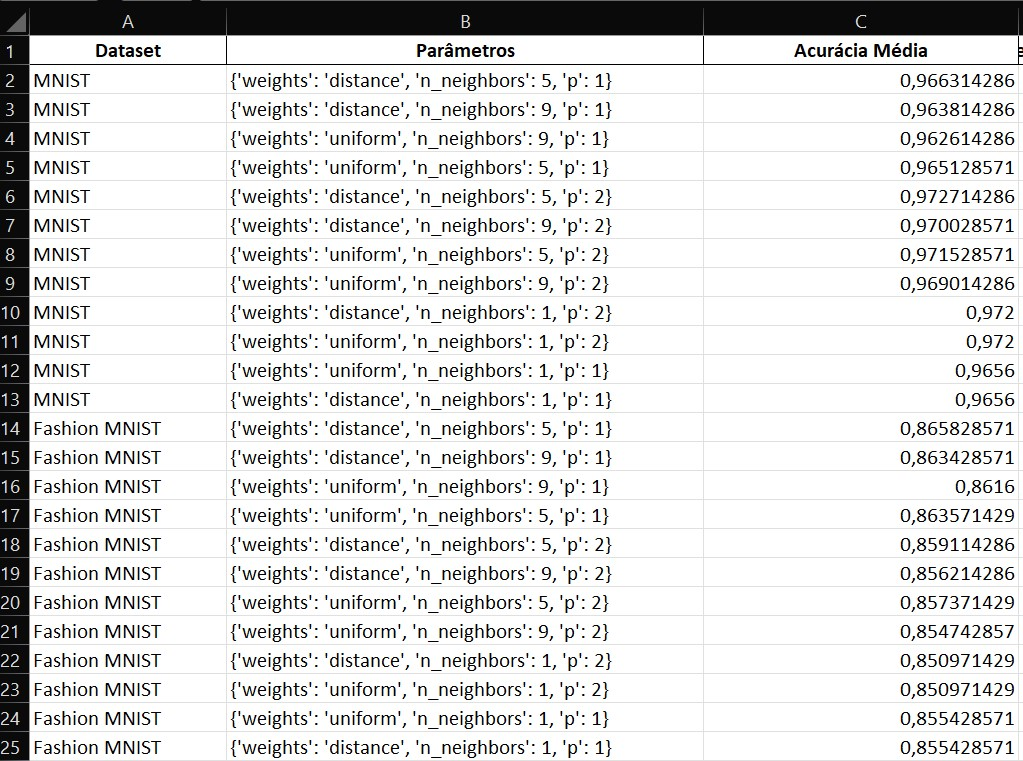
\includegraphics[width=0.8\textwidth]{knnplan01.jpg}
    \caption{Acurácias Médias da Reprodução}
    \label{fig:plan1}
\end{figure}

Os valores tabulados no artigo para esse mesmo classificador, conforme dados da página 4, estão disponíveis na figura abaixo:
\begin{figure}[H]
    \centering
    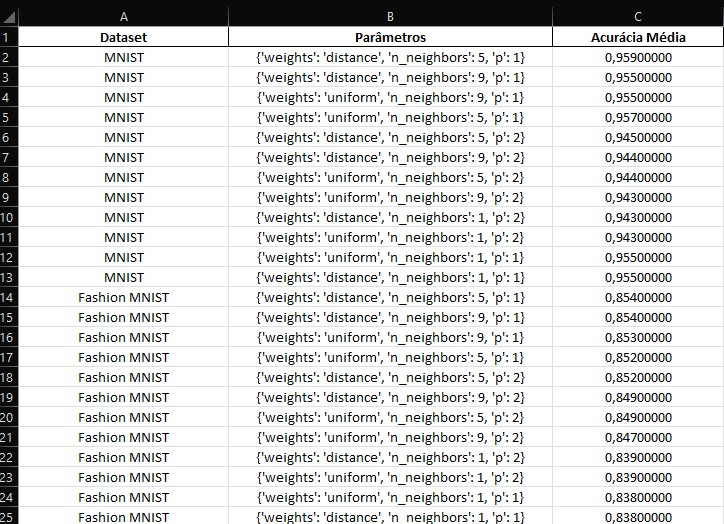
\includegraphics[width=0.8\textwidth]{knnplan02.jpg}
    \caption{Acurácias Médias do Artigo}
    \label{fig:plan2}
\end{figure}

\subsection{MLPClassifier}

Desenvolvemos um \textit{script} em \textit{python} acessível num repositório  em \url{https://github.com/deployrjrs/fpcc2/tree/master/mlp} onde está o código desse experimento que realiza o processamento do classificador \textit{MLPClassifier} sobre os dois \textit{datasets}, com o objetivo de verificar e registrar as acurácias médias dos experimentos, conforme  trabalho do paper original. 

Nesse experimento utilizamos os mesmos parâmetros do experimento original para o classificador acima, conforme consta na tabela abaixo:
\begin{table}[h]
\centering
\begin{tabular}{cc}
    \toprule
    \midrule
    \textbf{\#} & \textbf{Parâmetro} \\
    1 & $activation=relu, hidden\_layer\_sizes=[100]$  \\
    2 & $activation=relu, hidden\_layer\_sizes=[100, 10]$ \\
    3 & $activation=tanh, hidden\_layer\_sizes=[100] $ \\
    4 & $activation=tanh, hidden\_layer\_sizes=[100, 10]$ \\
    5 & $activation=relu, hidden\_layer\_sizes=[10, 10]$ \\
    6 & $activation=relu, hidden\_layer\_sizes=[10]$  \\
    7 & $activation=tanh, hidden\_layer\_sizes=[10, 10]$ \\
    8 & $activation=tanh, hidden\_layer\_sizes=[10]$ \\
\bottomrule
\end{tabular}
\caption{Parametrização MLPClassifier}
\label{tab:tabela2}
\end{table}

Na realização da reprodução desse experimento realizamos 5 execuções para cada uma das configurações de parâmetros para obter a média das acurácias. O que totalizou 80 execuções do algoritmo nos dois \textit{datasets}, com um tempo total de execução em máquina de 332 minutos e 52 segundos.

O resultado foi registrado pelo script em python na planilha resultados-benchmarkMLP em \url{https://github.com/deployrjrs/fpcc2/tree/master/mlp} que apresentamos na figura abaixo:
\begin{figure}[H]
    \centering
    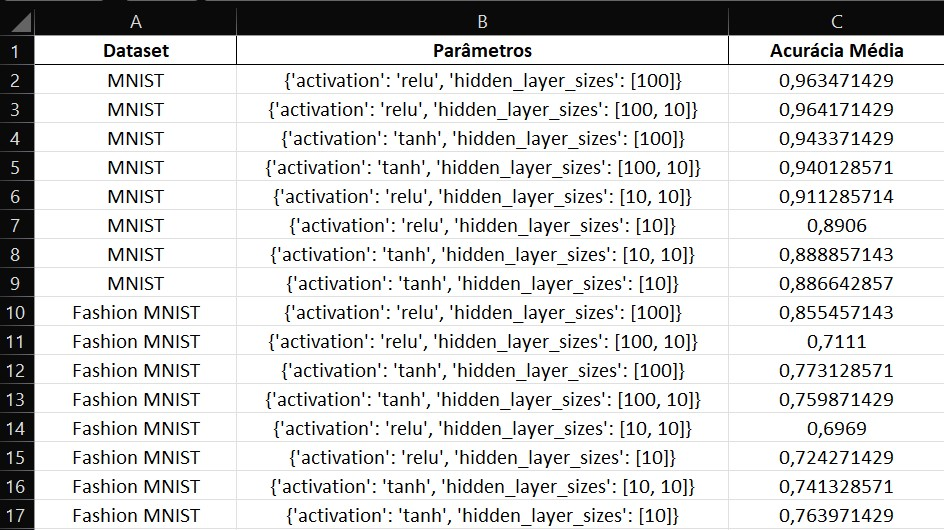
\includegraphics[width=0.8\textwidth]{mlpplan01.jpg}
    \caption{Acurácias Médias da Reprodução}
    \label{fig:planm1}
\end{figure}

Os valores tabulados no artigo para esse mesmo classificador, conforme dados da página 5, estão disponíveis na figura abaixo:
\begin{figure}[H]
    \centering
    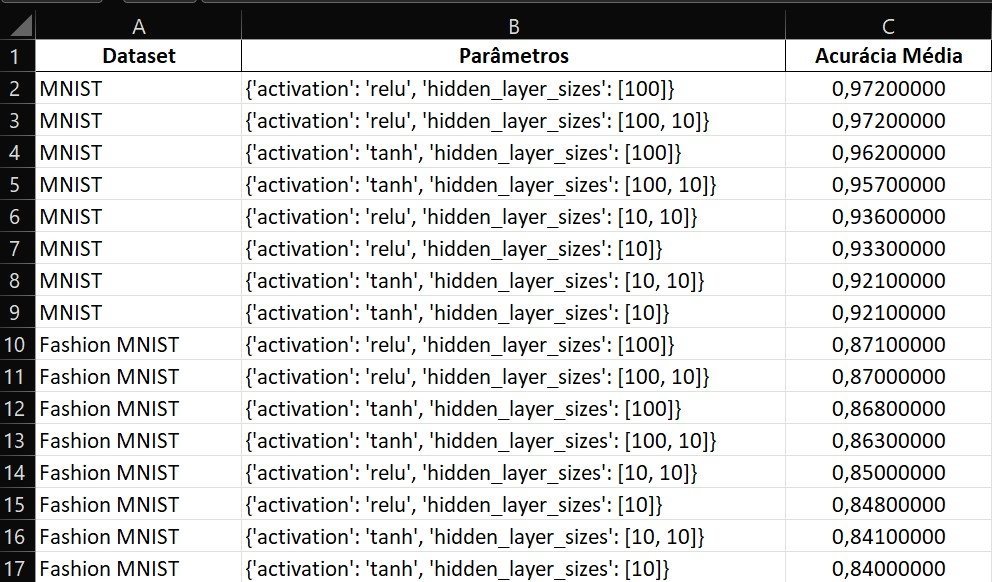
\includegraphics[width=0.8\textwidth]{mlpplan02.jpg}
    \caption{Acurácias Médias do Artigo}
    \label{fig:planm2}
\end{figure}


\subsection{LogisticRegression}

Desenvolvemos um \textit{script} em \textit{python} acessível num repositório  em \url{https://github.com/deployrjrs/fpcc2/tree/master/lr} onde consta o código desse experimento que realiza o processamento do classificador \textit{LogisticRegression} sobre os dois \textit{datasets}, com o objetivo de verificar e registrar as acurácias médias dos experimentos, conforme também fora realizado no trabalho original. 

Nesse experimento utilizamos os mesmos parâmetros do experimento original para o classificador acima, conforme consta na tabela abaixo:
\begin{table}[h]
\centering
\begin{tabular}{cc}
    \toprule
    \midrule
    \textbf{\#} & \textbf{Parâmetro} \\
    1 & $C=1, multi\_class=ovr, penalty=l1$   \\
    2 & $C=10, multi\_class=ovr, penalty=l2$  \\
    3 & $C=10, multi\_class=ovr, penalty=l2$  \\
    4 & $C=10, multi\_class=ovr, penalty=l1$ \\
    5 & $C=100, multi\_class=ovr, penalty=l2$ \\
\bottomrule
\end{tabular}
\caption{Parametrização LogisticRegression}
\label{tab:tabela3}
\end{table}

Na realização da reprodução desse experimento realizamos 5 execuções para cada uma das configurações de parâmetros para obter a média das acurácias. O que totalizou 50 execuções do algoritmo nos dois \textit{datasets}, com um tempo total de execução em máquina de 735 minutos e 24 segundos.

O resultado foi registrado pelo script em python na planilha resultados-benchmarkLRE em \url{https://github.com/deployrjrs/fpcc2/tree/master/lr} que apresentamos na figura abaixo:
\begin{figure}[H]
    \centering
    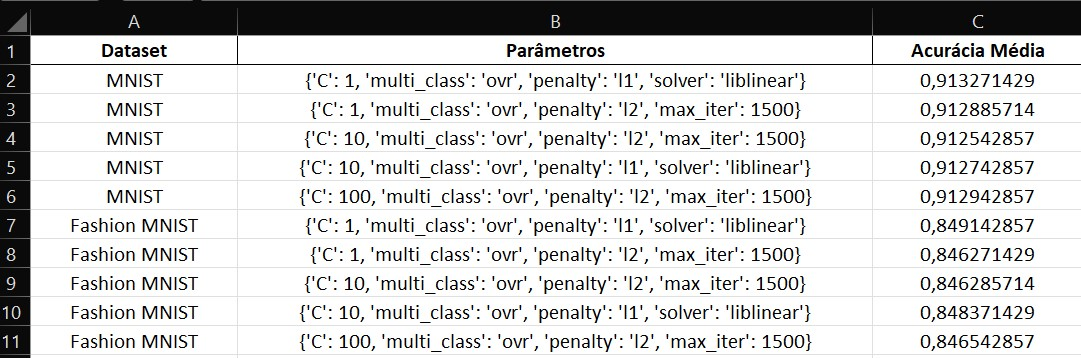
\includegraphics[width=0.8\textwidth]{lrplan01.jpg}
    \caption{Acurácias Médias da Reprodução}
    \label{fig:planlr1}
\end{figure}

Os valores tabulados no artigo para esse mesmo classificador, conforme dados da página 5, estão disponíveis na figura abaixo:
\begin{figure}[H]
    \centering
    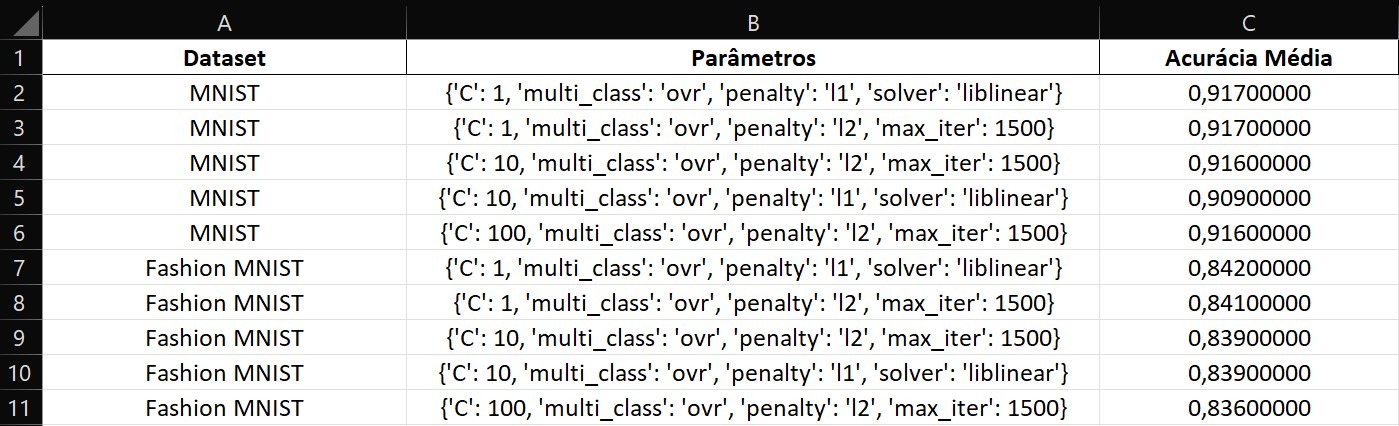
\includegraphics[width=0.8\textwidth]{lrplan02.jpg}
    \caption{Acurácias Médias do Artigo}
    \label{fig:planlr2}
\end{figure}

\section{Análise e Discussão}

Em nossa reprodução do artigo acrescentaremos uma análise estatística com o teste t independente (para amostras independentes) aplicado entre as diferenças das médias obtidas em cada experimento (de aplicar o mesmo algoritmo classificador no MNIST e no 
fashion MNIST), para testar as hipóteses sobre se houve ou não diferença estatiscamente significativa nas acurácias médias da classificação das imagens quando adotamos um ou outro \textit{dataset}.

Para avaliar as unidades de tratamento, desenvolvemos algoritmos em python que verificam as condições de aplicação do teste t independente, checando a normalidade dos dados num vetor que guarda a diferença entre as médias, para cada experimento com um classificador sobre os dois datasets e em seguida aplicamos um teste de hipóteses com base nas estatísticas do t independente. 

Adotamos como hipótese nula $H_0$ que 'não há diferença significativa entres as médias das acurácias' calculadas sobre o MNIST e sobre o fashion MNIST, pelo classificador. Como hipótese alternativa $H_a$ testamos se 'há diferença significativa entre as médias das acurácias' calculadas sobre o MNIST e sobre o fashion MNIST, pelo classificador.


\subsection{t Independente para o KNeighborsClassifier}
Abaixo apresentamos a figura com os resultados do teste t independente executado pelos scripts e dados dos experimentos realizados em\url{https://github.com/deployrjrs/fpcc2/tree/master/stats} para o classificador KNeighborsClassifier utilizado nessa reprodução.
\begin{figure}[H]
    \centering
    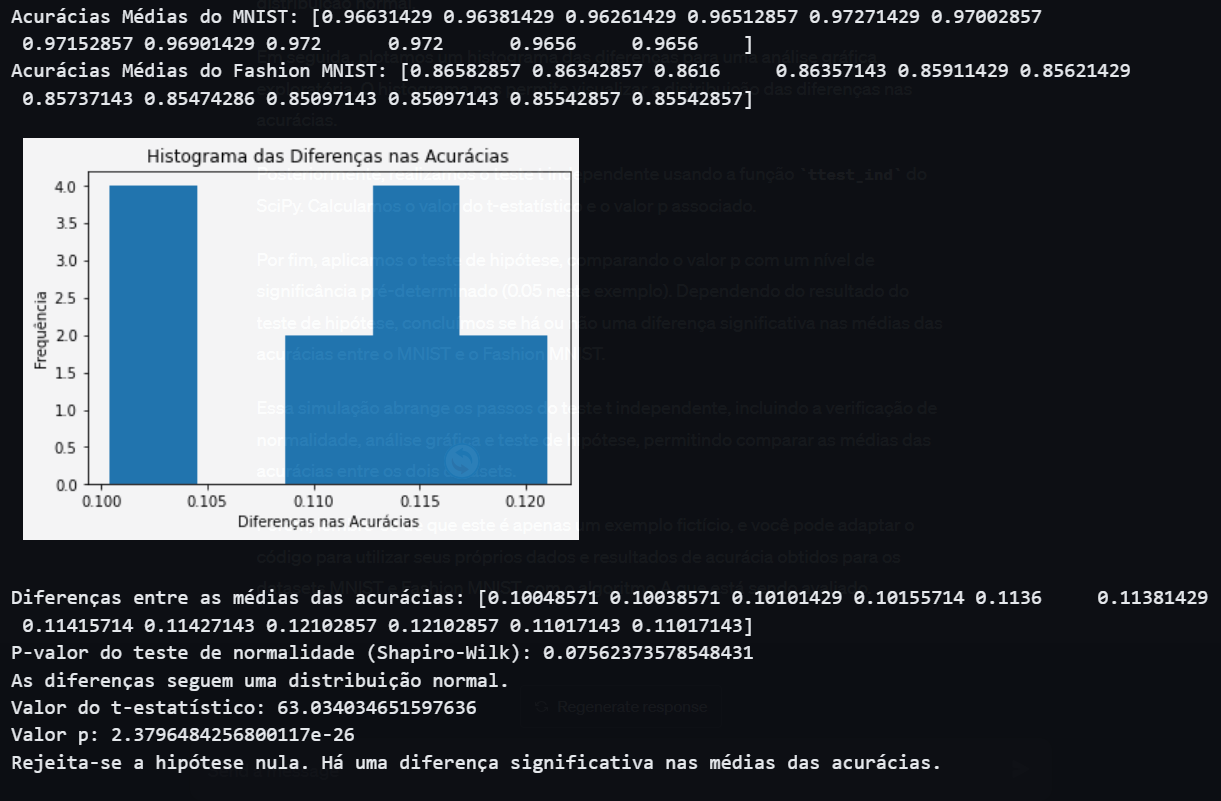
\includegraphics[width=1.0\textwidth]{KNstats.png}
    \caption{Resultado do t Independente para o KNeighborsClassifier}
    \label{fig:knstats}
\end{figure}

\subsection{t Independente para o MLPClassifier}
Abaixo apresentamos a figura com os resultados do teste t indepedente executado pelos scripts e dados dos experimentos realizados em\url{https://github.com/deployrjrs/fpcc2/tree/master/stats} para o classificador MLPClassifier utilizado nessa reprodução.
\begin{figure}[H]
    \centering
    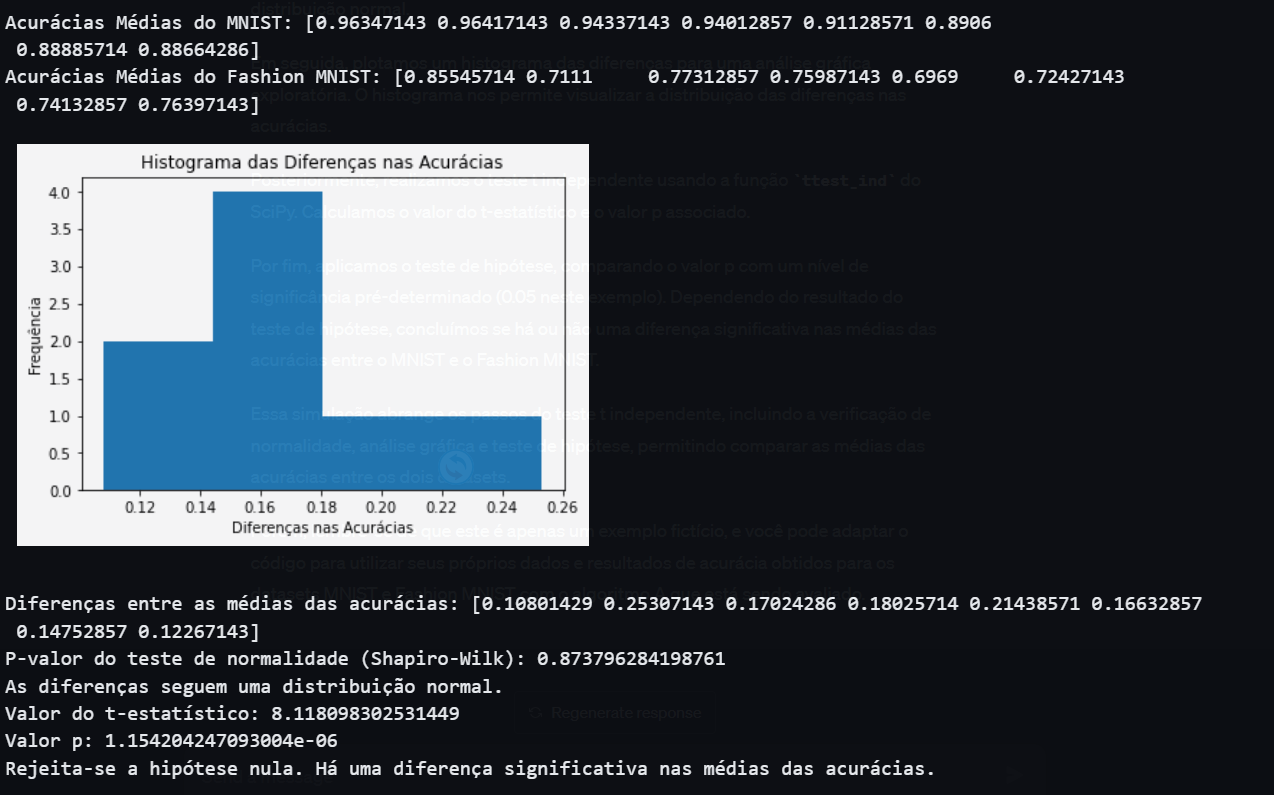
\includegraphics[width=1.0\textwidth]{MLPstats.png}
    \caption{Resultado do t Independente para o MLPClassifier}
    \label{fig:knstats}
\end{figure}

\subsection{t Independente para o LogisticRegression}
Abaixo apresentamos a figura com os resultados do teste t independente executado pelos scripts e dados dos experimentos realizados em\url{https://github.com/deployrjrs/fpcc2/tree/master/stats} para o classificador LogisticRegression utilizado nessa reprodução.
\begin{figure}[H]
    \centering
    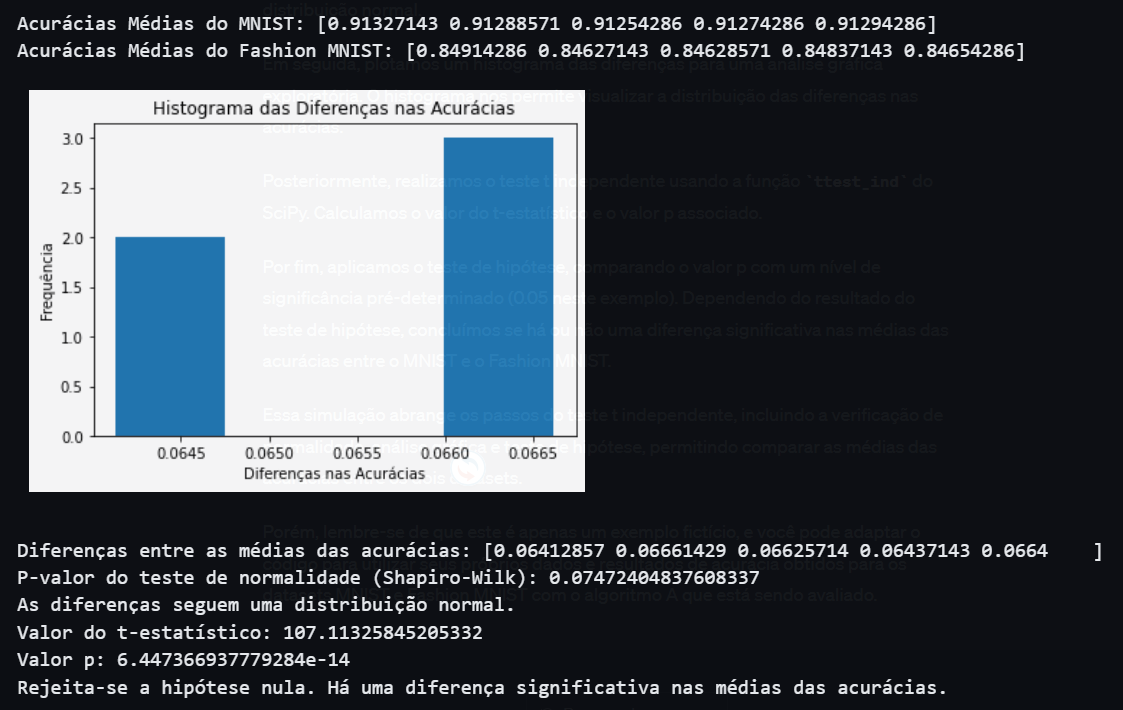
\includegraphics[width=1.0\textwidth]{LRstats.png}
    \caption{Resultado do t Independente para o LogisticRegression}
    \label{fig:lrstats}
\end{figure}

Com essa análise estatística efetuada, de fato podemos afirmar que as evidências apontam que o \textit{dataset} fashion MNIST é mais desafiador em termos de classificação de imagens. Ou seja, é mais próximo do mundo real devido a sua
grande variabilidade das classes de imagens que apresenta, sendo portanto um \textit{dataset} apropriado não somente para testes e análises de problemas de classificação associados ao domínio da moda, como também em outros domínios.\cite{Olivia}.

\section{Conclusão}

Nesse relatório de reprodutibilidade fizemos a reprodução do artigo \cite{Xiao2017FashionMNISTAN}, definindo um recorte de pesquisa que considerou três dos classificadores usados no artigo original, mantendo-se os mesmos parâmetros e quantidades de testes efetuados sobre os dois \textit{datasets} considerados. Desenvolvemos um conjunto de scripts em python usando a biblioteca Scikit Learn e os classificadores em questão, para conduzir os experimentos de reprodutibilidade e consideramos uma análise da significância estatística dos resultados obtidos nessa reprodução, dando evidências de que o 'Fashion MNIST' é um dataset mais apropriado para testes de classificação de imagens, não apenas para a indústria da moda, mas para testar outros algoritmos de classificação de imagens outros domínios distintos da moda. Todos os dados dessa reprodução foram tornados públicos em \url{https://github.com/deployrjrs/fpcc2/tree/master/} para exames, consulltas e reprodução.
%%\bibliographystyle{alpha}
\bibliographystyle{ieeetr}
\bibliography{repro.bib}
\end{document}
